%----------------------------------------------------------------------------------------
% METADATA BLOCK (YAML)  — see inbox/README.md for every field
%----------------------------------------------------------------------------------------
% uid: ""
% school: "lycee"
% level: "3eme"
% section: "Mathématiques"
% chapter: "Trigonométrie"
% title: "Le théorème de Morley"
% difficulty: "Difficile"
% tags: ["morley", "trisectrices", "loi-des-sinus", "triangle-equilateral", "formule-de-triplication"]
% provenance: "adapted"
% batch: "2026-11-20-defis-geometrie-A"
%----------------------------------------------------------------------------------------

% ---STATEMENT---
Soit $ABC$ un triangle dont les angles sont $\widehat A=3\alpha$, $\widehat B=3\beta$, $\widehat C=3\gamma$, avec $\alpha+\beta+\gamma=60^\circ$. On note $R$ le rayon de son cercle circonscrit. On trace les six trisectrices des angles du triangle. On appelle
\begin{itemize}
  \item $D$ le point d'intersection des trisectrices issues de $B$ et de $C$ qui sont les plus proches de $[BC]$,
  \item $E$ le point d'intersection des trisectrices issues de $C$ et de $A$ les plus proches de $[CA]$,
  \item $F$ le point d'intersection des trisectrices issues de $A$ et de $B$ les plus proches de $[AB]$.
\end{itemize}

% alt: Triangle ABC avec ses six trisectrices ; D, E, F : intersections des trisectrices adjacentes aux côtés BC, CA, AB
\begin{center}
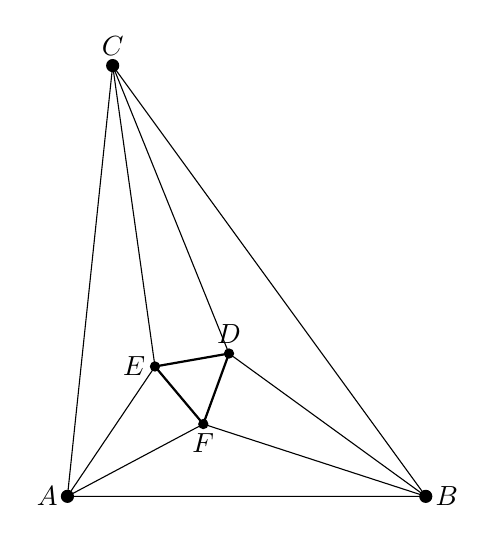
\begin{tikzpicture}[scale=1.7,line cap=round,line join=round,>=stealth]
\draw (0,0) -- (2.677,0) -- (0.338,3.218) -- cycle;
\draw[thin] (0,0) -- (1.015,0.54);
\draw[thin] (0,0) -- (0.654,0.97);
\draw[thin] (2.677,0) -- (1.015,0.54);
\draw[thin] (2.677,0) -- (1.207,1.067);
\draw[thin] (0.338,3.218) -- (0.654,0.97);
\draw[thin] (0.338,3.218) -- (1.207,1.067);
\draw[thick] (1.207,1.067) -- (0.654,0.97) -- (1.015,0.54) -- cycle;
\fill(0,0) circle (1.4pt) node[left] {$A$};
\fill(2.677,0) circle (1.4pt) node[right] {$B$};
\fill(0.338,3.218) circle (1.4pt) node[above] {$C$};
\fill(1.207,1.067) circle (1.1pt) node[above] {$D$};
\fill(0.654,0.97) circle (1.1pt) node[left] {$E$};
\fill(1.015,0.54) circle (1.1pt) node[below] {$F$};
\end{tikzpicture}
\end{center}

On veut montrer que \textbf{le triangle $DEF$ est équilatéral}.
\begin{enumerate}
  \item Montrer que pour tout réel $x$ : $\sin3x=4\sin x\,\sin(60^\circ-x)\,\sin(60^\circ+x)$.
  \item Dans le triangle $ABF$, puis dans le triangle $ACE$, exprimer $AF$ et $AE$ à l'aide de la loi des sinus et de $AB=2R\sin3\gamma$, $AC=2R\sin3\beta$. Montrer que
  \[AF=8R\sin\beta\sin\gamma\sin(60^\circ+\gamma),\qquad AE=8R\sin\beta\sin\gamma\sin(60^\circ+\beta).\]
  \item Soient $X$, $Y$, $Z$ trois angles tels que $X+Y+Z=180^\circ$. Montrer que $\sin^2X+\sin^2Y-2\sin X\sin Y\cos Z=\sin^2Z$.
  \item En appliquant la loi des cosinus dans le triangle $AEF$ (où $\widehat{EAF}=\alpha$), montrer que $EF=8R\sin\alpha\sin\beta\sin\gamma$, puis conclure.
\end{enumerate}

% ---SOLUTION---
\begin{enumerate}[itemsep=14pt]
  \item\leavevmode
  \begin{prop}[Formules d'addition]
  \textbf{$\sin(a\pm b)=\sin a\cos b\pm\cos a\sin b$}\quad et\quad \textbf{$\cos(a\pm b)=\cos a\cos b\mp\sin a\sin b$}.
  \end{prop}
  Calculons le produit $\sin(60^\circ-x)\sin(60^\circ+x)$ avec $\sin a\sin b=\dfrac12[\cos(a-b)-\cos(a+b)]$ :
  \[\begin{aligned}\sin(60^\circ-x)\sin(60^\circ+x)&=\dfrac12\big[\cos(2x)-\cos120^\circ\big]=\dfrac12\left[\cos2x+\dfrac12\right]\\ &=\dfrac12\left[1-2\sin^2x+\dfrac12\right]=\dfrac34-\sin^2x.\end{aligned}\]
  Donc
  \[4\sin x\,\sin(60^\circ-x)\sin(60^\circ+x)=4\sin x\left(\dfrac34-\sin^2x\right)=3\sin x-4\sin^3x=\sin3x.\]
  (formule de triplication $\sin3x=3\sin x-4\sin^3x$).

  \item\leavevmode
  \begin{prop}[Loi des sinus]
  Dans un triangle de côtés $a,b,c$ et d'angles opposés $\hat A,\hat B,\hat C$ : \textbf{$\dfrac{a}{\sin\hat A}=\dfrac b{\sin\hat B}=\dfrac c{\sin\hat C}$}, et ce rapport vaut $2R$.
  \end{prop}
  Dans $ABF$ : l'angle en $A$ vaut $\alpha$, l'angle en $B$ vaut $\beta$, donc l'angle en $F$ vaut $180^\circ-(\alpha+\beta)$, de sinus $\sin(\alpha+\beta)$. Avec $\alpha+\beta=60^\circ-\gamma$ :
  \[\dfrac{AF}{\sin\beta}=\dfrac{AB}{\sin(60^\circ-\gamma)}\iff AF=\dfrac{2R\sin3\gamma\,\sin\beta}{\sin(60^\circ-\gamma)}.\]
  D'après la question 1, $\sin3\gamma=4\sin\gamma\sin(60^\circ-\gamma)\sin(60^\circ+\gamma)$ ; on simplifie par $\sin(60^\circ-\gamma)$ :
  \[\ib{$AF=8R\sin\beta\sin\gamma\sin(60^\circ+\gamma)$}.\]
  Dans $ACE$ : l'angle en $A$ vaut $\alpha$, l'angle en $C$ vaut $\gamma$, l'angle en $E$ vaut $180^\circ-(\alpha+\gamma)$ et $\alpha+\gamma=60^\circ-\beta$ :
  \[\dfrac{AE}{\sin\gamma}=\dfrac{AC}{\sin(60^\circ-\beta)}\iff AE=\dfrac{2R\sin3\beta\,\sin\gamma}{\sin(60^\circ-\beta)}=\ib{$8R\sin\beta\sin\gamma\sin(60^\circ+\beta)$}.\]

  \item\leavevmode
  \begin{prop}[Loi des cosinus]
  Dans un triangle, \ib{$a^2=b^2+c^2-2bc\cos\hat A$}.
  \end{prop}
  Soit un triangle d'angles $X$, $Y$, $Z$ (somme $180^\circ$), inscrit dans un cercle de diamètre $1$ : ses côtés sont $\sin X$, $\sin Y$, $\sin Z$. La loi des cosinus donne $\sin^2Z=\sin^2X+\sin^2Y-2\sin X\sin Y\cos Z$.

  \emph{(Autre preuve, sans triangle :)} $Z=180^\circ-(X+Y)$ donc $\cos Z=-\cos(X+Y)$ et $\sin Z=\sin(X+Y)$ ; on développe $\sin^2(X+Y)$ et on compare.

  \item Dans $AEF$, l'angle en $A$ est celui entre les deux trisectrices qui encadrent le tiers du milieu : $\widehat{EAF}=\alpha$.

  \[\begin{aligned}EF^2&=AE^2+AF^2-2\,AE\cdot AF\cos\alpha\\ &=(8R\sin\beta\sin\gamma)^2\Big[\sin^2(60^\circ+\beta)+\sin^2(60^\circ+\gamma)-2\sin(60^\circ+\beta)\sin(60^\circ+\gamma)\cos\alpha\Big].\end{aligned}\]
  Prenons $X=60^\circ+\beta$, $Y=60^\circ+\gamma$, $Z=\alpha$ : $X+Y+Z=120^\circ+(\alpha+\beta+\gamma)=180^\circ$. D'après la question 3, le crochet vaut $\sin^2\alpha$. Donc
  \[EF^2=(8R\sin\alpha\sin\beta\sin\gamma)^2,\qquad\ib{$EF=8R\sin\alpha\sin\beta\sin\gamma$}.\]
  L'expression est \emph{symétrique} en $\alpha,\beta,\gamma$. Le même raisonnement fait au sommet $B$ donne $FD=8R\sin\alpha\sin\beta\sin\gamma$ et au sommet $C$, $DE=8R\sin\alpha\sin\beta\sin\gamma$.

  Donc $DE=EF=FD$ : \ib{le triangle $DEF$ est équilatéral}. $\blacksquare$
\end{enumerate}

\textbf{Idée :} la formule de triplication $\sin3x=4\sin x\sin(60^\circ-x)\sin(60^\circ+x)$ fait apparaître $\sin(60^\circ+\cdot)$ ; les trois angles $\alpha$, $60^\circ+\beta$, $60^\circ+\gamma$ sont ceux d'un vrai triangle, ce qui permet de refermer le calcul de $EF$ avec la loi des cosinus.

\textbf{Piège :} les trisectrices \emph{adjacentes} à un côté sont celles qui forment, avec ce côté, les angles $\beta,\gamma$ (et non $2\beta$, $2\gamma$) ; sinon $AF$ et $AE$ ne sont pas ceux calculés ici.

\textbf{Pour aller plus loin.} Conway a donné une preuve sans calcul : on construit un triangle équilatéral central, on lui accole six triangles d'angles convenables, puis on montre que la figure obtenue est semblable à $ABC$.
